\section{Experiment}

The analysis was completed in Python, and the hierarchical Bayesian model built in Python using the PyMC package \cite{pymc2023}. 

First, the data set was processed following section \ref{sec:dataoverview}. Early cycle features described in table \ref{table:features} were extracted and the data was partitioned into 8 groups like described in section \ref{subsec:GroupingResults}. The following experiment was completed using the grouping using the hill-climbing algorithm, because a high VPC justifies the use of a hierarchical model since group level effect would be significant. If the authors grouping method was used in this analysis with our data set, the VPC was only 39\% and the results of the hierarchical Baysian model would not be significantly.

The data was randomly split into a training and test dataset, with 135 cells in training set and 34 cell in the test set. The train-test split was stratified on the cycling group $g$, ensuring that the model will encounter the same proportions of cells from each cycling condition group. On the training set, a 5-fold cross validation was performed 4 times (so 20 results will be collected) to ensure that the model is not overfitting to the dataset. After that, the model was fit to the whole training set and evaluated using the unseen test set.

\section{Results and Discussion}

The performance of the Hierarchical Bayesian model is compared against two baselines: a ridge regression model with just the features in Table \ref{table:features}, and one including the cycling group $g$ as well. Root mean error squared (RMSE) and mean absolute percentage error (MAPE) are used as metrics to evaluate the performance of the models. We consider MAPE as an additional metric because RMSE is significantly influenced by outliers.
\begin{align*}
    \text{RMSE} &= \sqrt{\frac{\sum^N_{i=1} (y_i - \hat{y}_i)^2}{N}} \\
    \text{MAPE} &= \frac{1}{N}\sum^N_{i=1} \left| \frac{y_i - \hat{y}_i}{y_i} \right|
\end{align*}

\begin{table}[!ht]
\centering
\begin{tabular}{cccc}
\hline
             &   Baseline (without $g$) & Baseline (with $g$) &     HBM     \\
\hline
     RMSE    &    9.31                 &    6.51             &     7.23    \\
     MAPE    &    22.5\%                &    16.8\%           &     14.7\%  \\
\hline
\end{tabular}
\caption{Average RMSE (in days) and MAPE of the EoL predictions on the cross validation}
\label{table:RMSEandMAPE}
\end{table}

\begin{figure}[!ht]
    \centering
    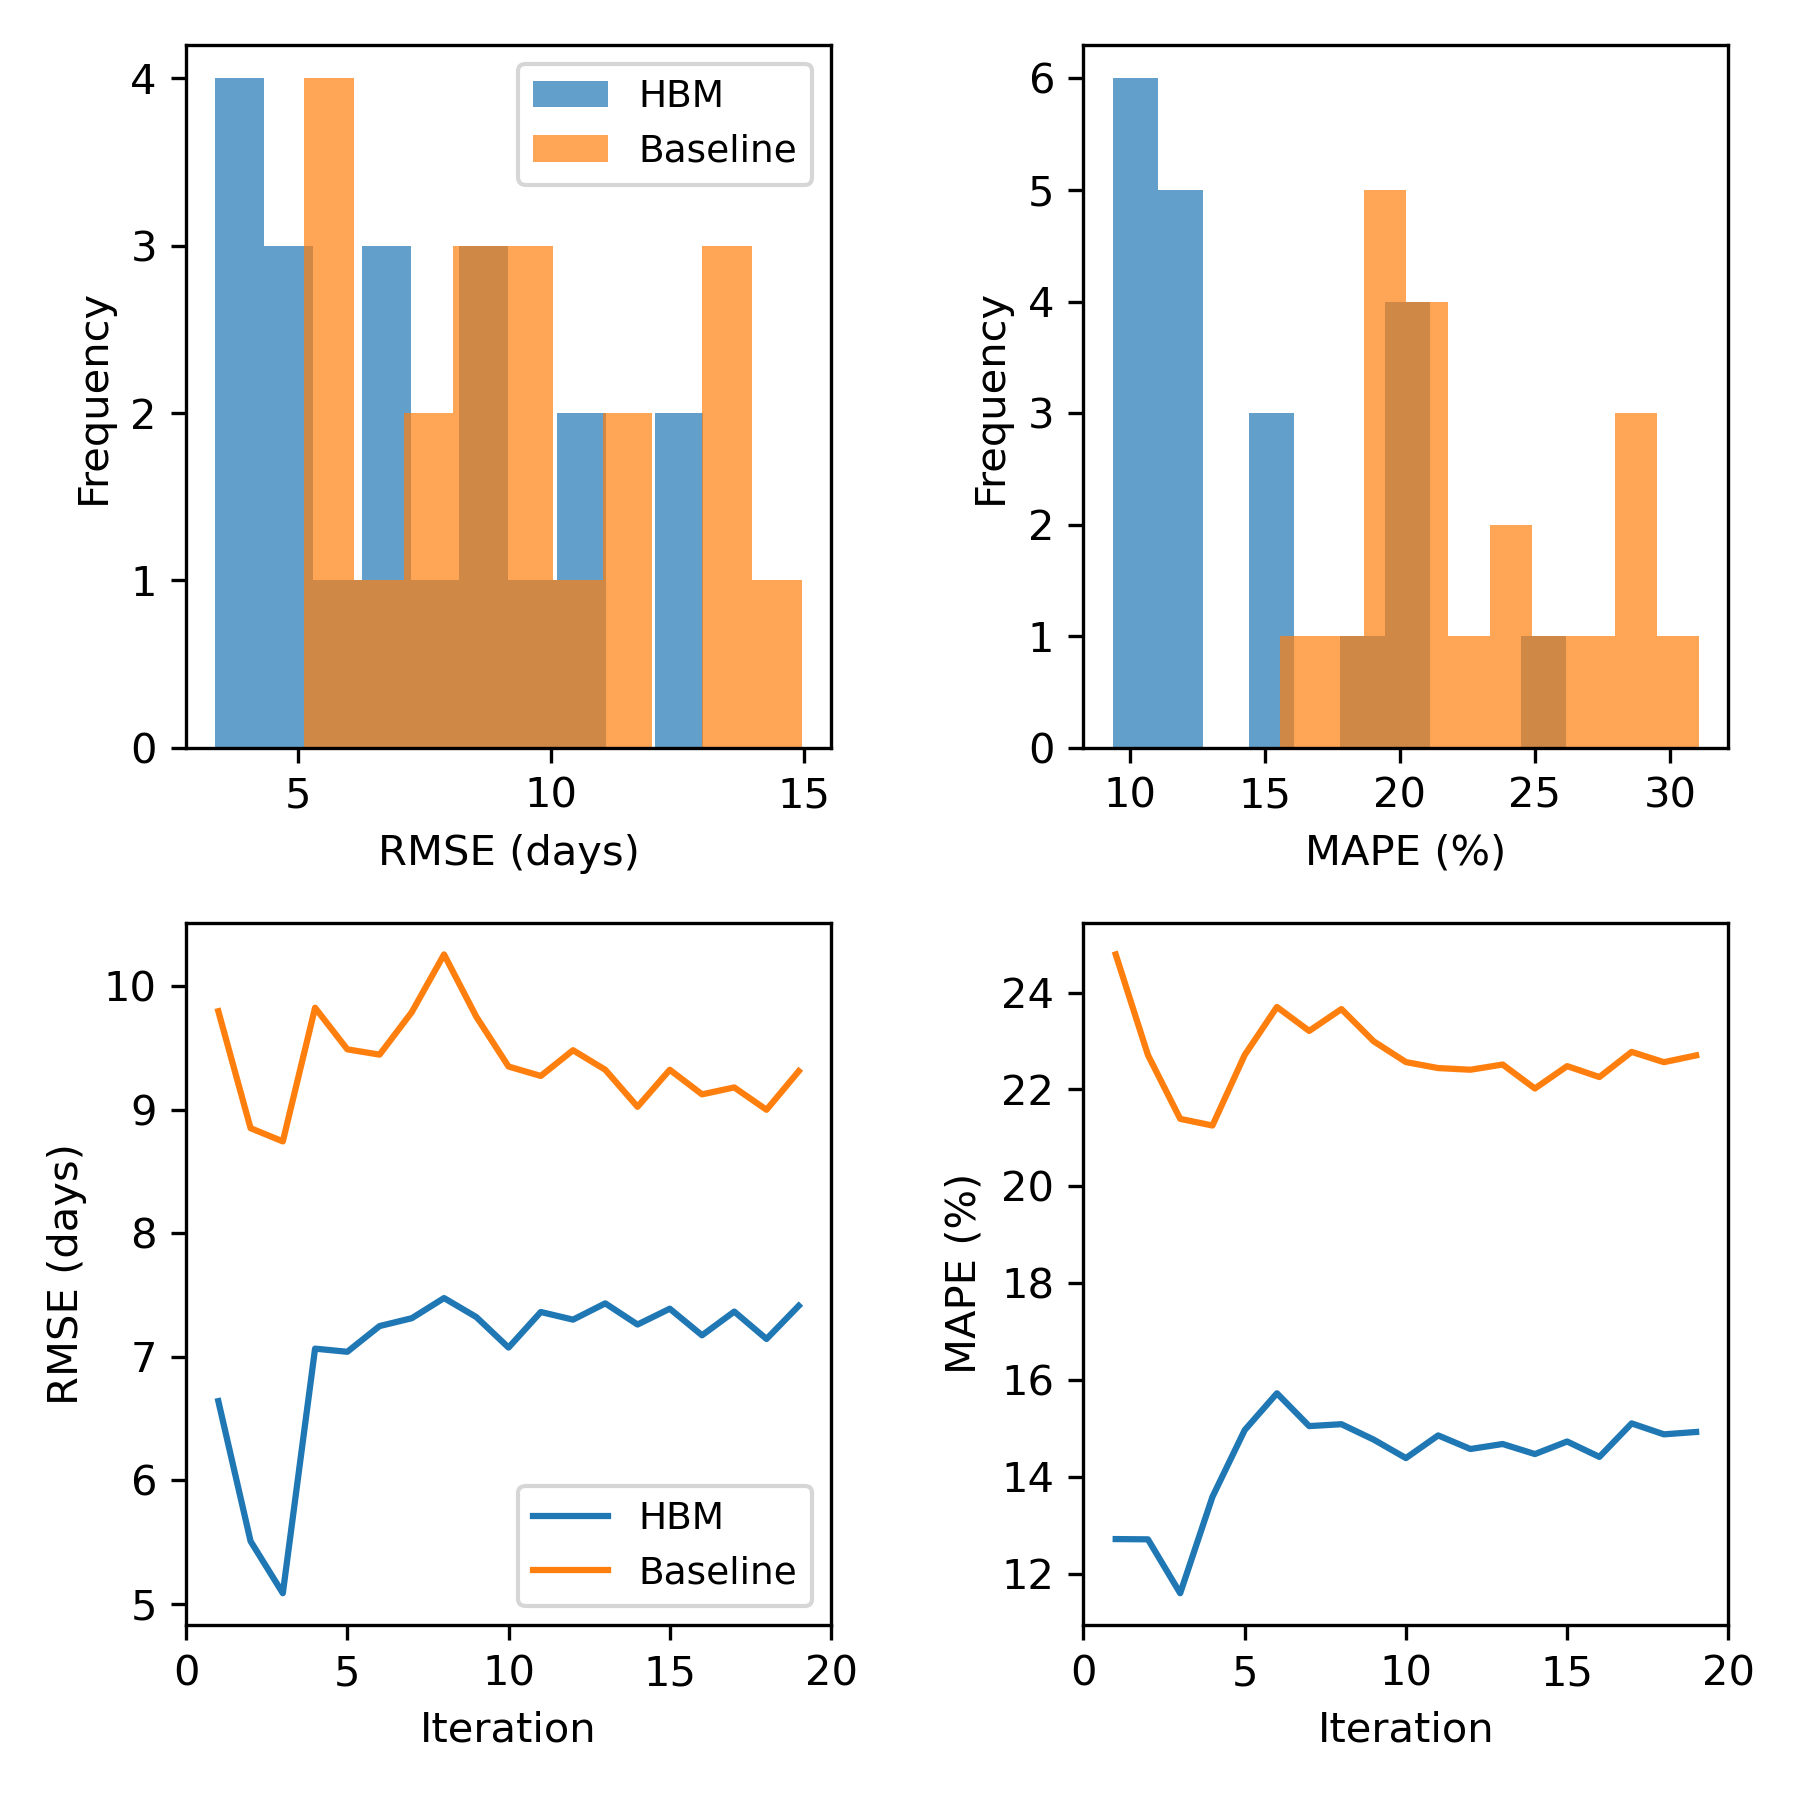
\includegraphics[width=0.75\linewidth]{kfolds_results.png}
    \caption{Histogram of all RSME and MAPE results for the HBM and baseline}
    \label{fig:kfolds_results}
\end{figure}

Table \ref{table:RMSEandMAPE} shows the average RMSE and MAPE after each repetition and fold, and figure \ref{fig:kfolds_results} shows the RMSE and MAPE values for each fold and repetition. HBM outperforms the baseline by $28.7\%$ with RMSE, but has similar results to the baseline with $g$ as a feature. This indicates the importance of the cycling condition as a feature and motivates the consideration of a hierarchical model, since conventional regression would treat the cycling condition and other features the same. Additionally, HBM outperforms both baseline models when considering MAPE. 

\begin{figure}[!ht]
    \centering
    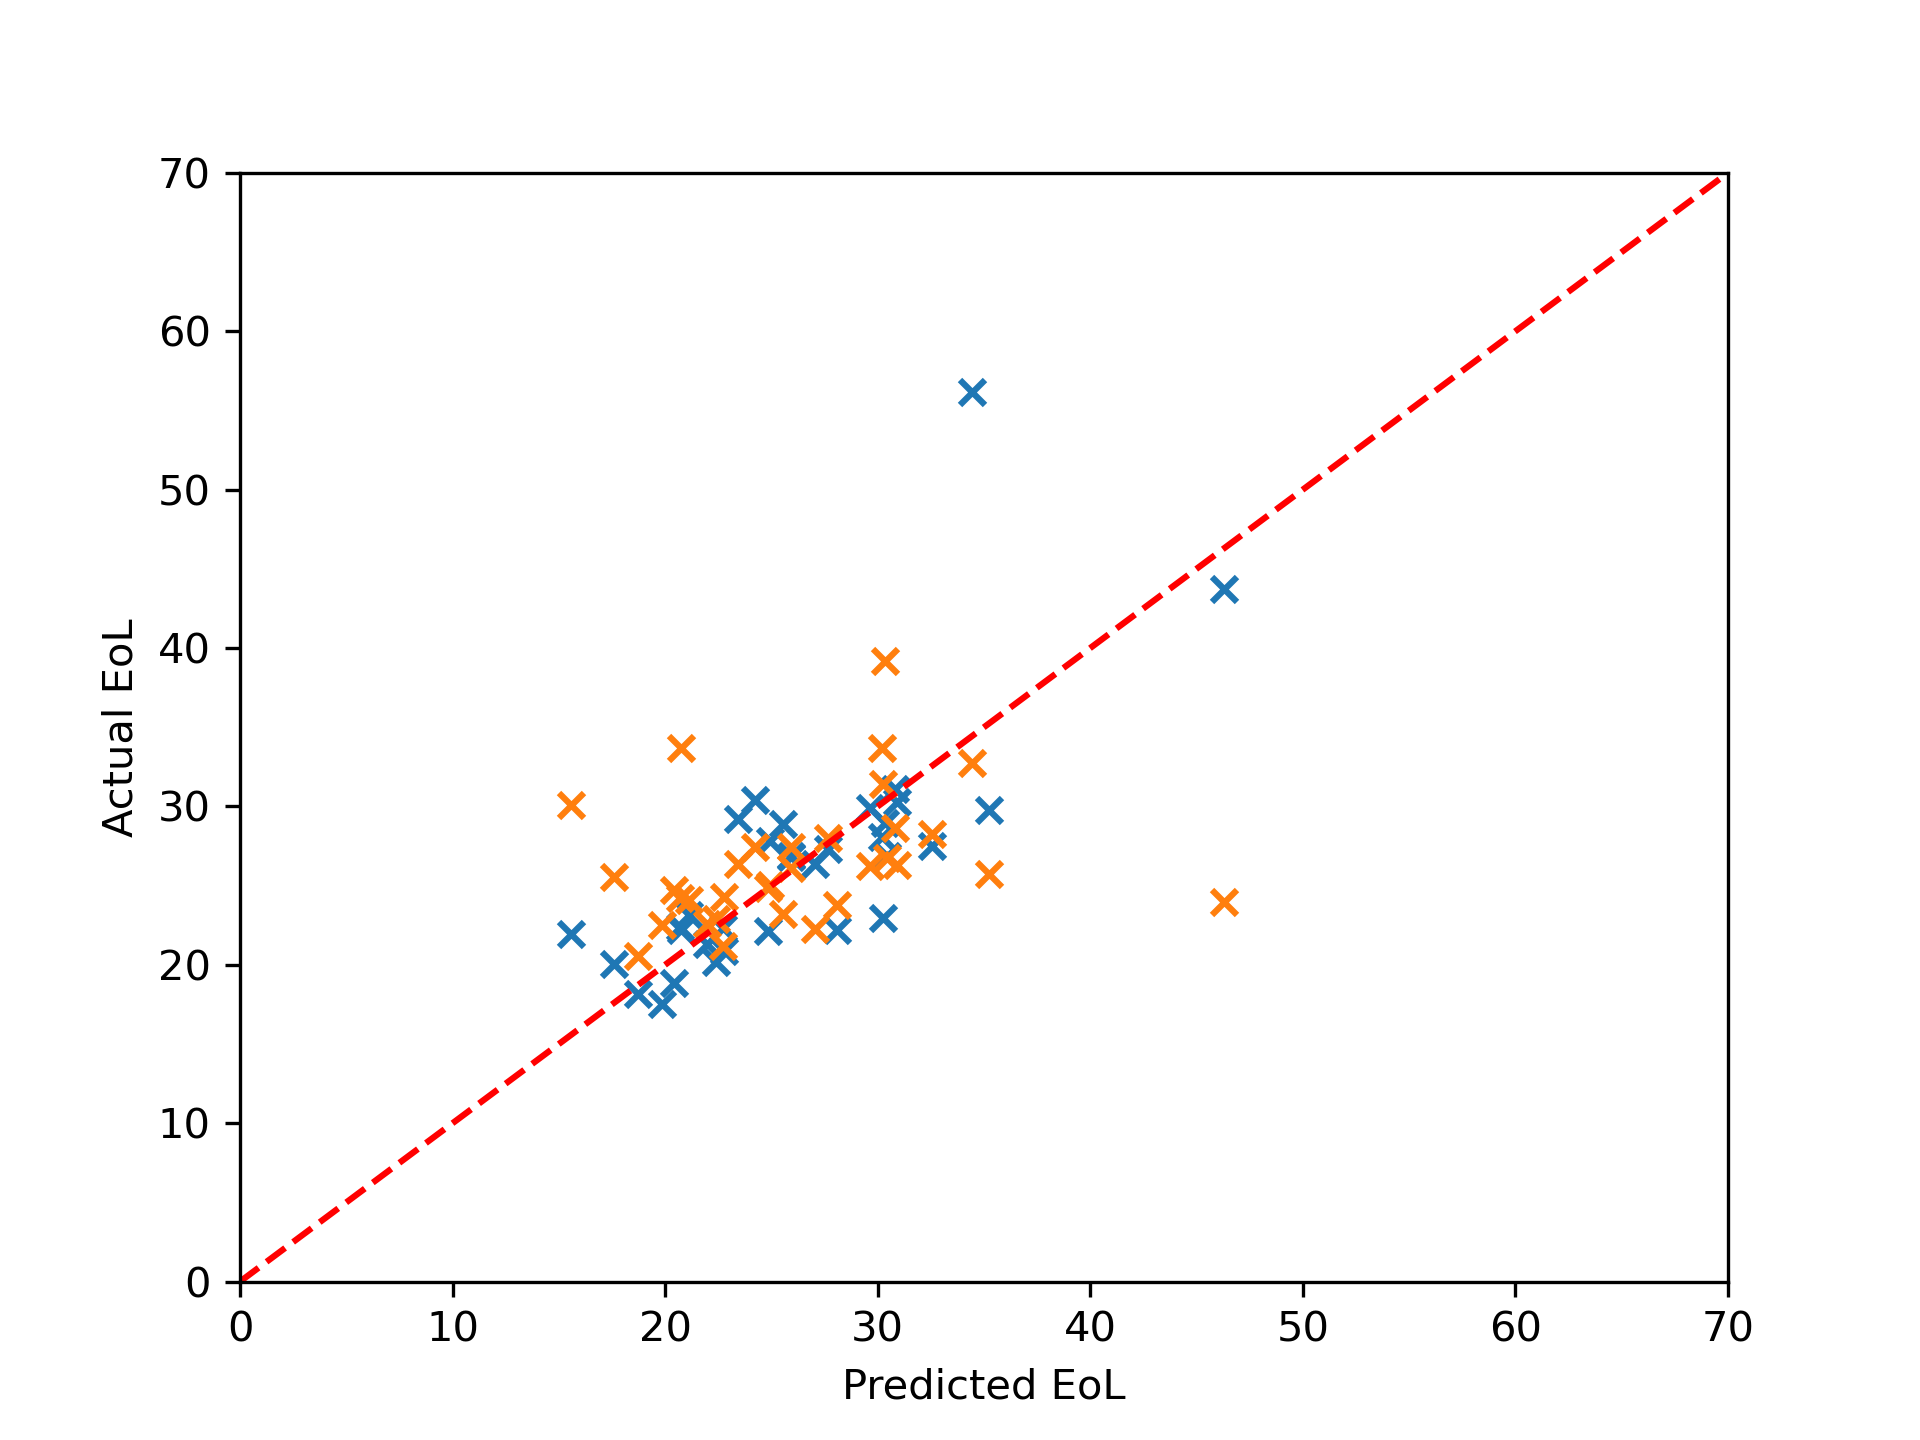
\includegraphics[width=0.75\linewidth]{results_scatterplot.png}
    \caption{Predicted v.s. actual EoL for HBM and baseline}
    \label{fig:results_scatterplot}
\end{figure}

\begin{table}[!ht]
\centering
\begin{tabular}{cccc}
\hline
             &   Baseline (without $g$) & Baseline (with $g$) &     HBM     \\
\hline
     RMSE    &    18.2                  &    18.2             &     18.8    \\
     MAPE    &    18.5\%                &    17.1\%           &     13.9\%  \\
\hline
\end{tabular}
\caption{RMSE (in days) and MAPE of the EoL predictions on the test set}
\label{table:finalRMSEandMAPE}
\end{table}

Now using just a training and test set, table \ref{table:finalRMSEandMAPE} shows the RMSE and MAPE on the test set predictions and figure \ref{fig:results_scatterplot} shows the EoL predictions from the HBM and baseline models compared to the true values.